\label{monitoramento_servicos}

Neste capítulo são apresentadas informações decorrentes da realização do monitoramento do barramento de serviços utilizando o Protocolo \acrshort{SNMP}. Na Seção \ref{recursos_monitoramento} é a apresentado o monitoramento dos recursos do barramento de serviços. Na Seção \ref{integracao_snmp} são apresentados alguns detalhes para a implantação do protocolo \acrshort{SNMP}. Na Seção \ref{metricas_monitoramento} são apresentadas as métricas adotadas para a realização do monitoramento do barramento. Na Seção ('\ ref') é apresentado o ......

\section{Monitoramento dos recursos do barramento de serviços}%
\label{recursos_monitoramento}

O \acrshort{CPD} da \acrshort{UnB} adotou como solução para a modernização, migração dos sistemas e tecnologia a implementação de uma arquitetura orientada a serviços, que vem sendo bastante utilizada principalmente para criação de serviços (\textit{web services}). A implementação dos serviços tem aumentado, devido a flexibilidade definida na arquitetura e o aumento da demanda para a realização de integração de sistemas, além da curva de aprendizagem ser alta. Com a implementação e disponibilização de  vários serviços, monitorar e acompanhar o funcionamento, tem se tornado uma tarefa que tem demandado um grande esforço das equipes de 
desenvolvimento do \acrshort{CPD}. O monitoramento do barramento de serviços da \acrshort{UnB} é realizado de três formas conhecidas, uma por meio do \textit{Log} de arquivos gerado pelo próprio barramento, onde as informações de registros do \textit{Log} são coletadas e apresentadas em um \textit{dashboard} de acordo com a figura \ref{fun:fig:dashboardS} \cite{filgueirasmonitoramento}, outra por meio de serviços (\textit{web services}) providos pelo barramento conforme a figura \ref{fun:fig:memoriaEMS}, além da nativa que é disponibilizada pela empresa que mantém e gerencia a linguagem Erlang, esse monitoramento é realizado pelo denominado \textit{Observer} que dispõe de elementos gráficos como apresentado na figura \ref{fun:fig:observer} para observar as características dos sistemas desenvolvidos em Erlang \cite{ericssonAB2002-2019}. 

\begin{figure}[h!]
	\begin{center}
	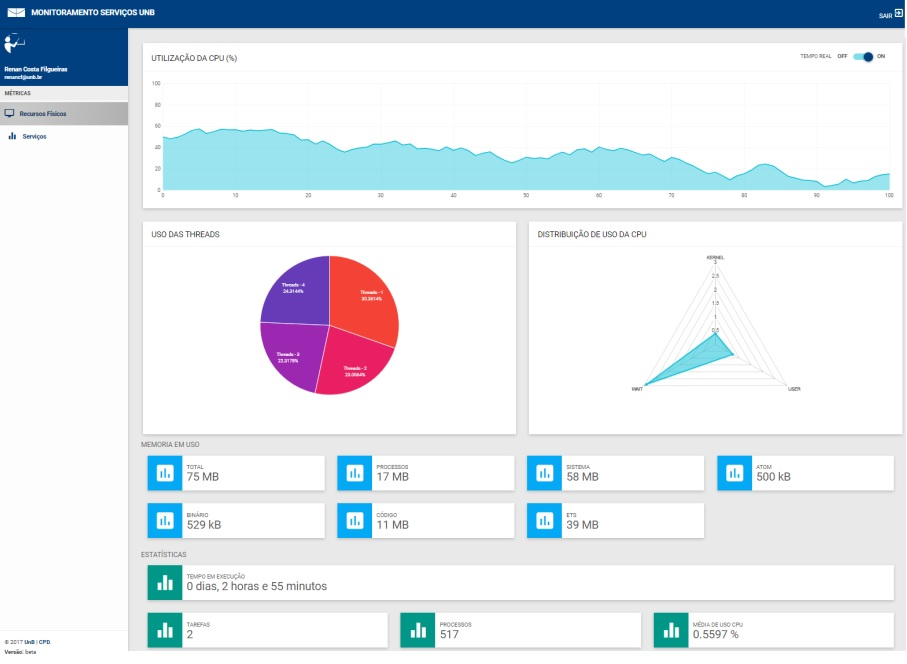
\includegraphics[scale = 0.70]{img/dashboard.jpg}
		\caption{\textit{Dashborad} de monitoramento \cite{filgueirasmonitoramento}}
		\label{fun:fig:dashboardS}
	\end{center}
\end{figure}

Este trabalho inclui uma nova forma de monitoramento para o barramento de serviços, esse monitoramento difere dos demais pelo modo de atuação, onde o foco é monitorar o funcionamento dos recuros que o barramento de serviços provém, desde o recurso responsável pelo registro das informações de \textit{Log} passando pelo os recursos que executam os processos de autenticação e autorização até o recurso responsável pelo recebimento e transmissão de requisições. Devido a escolha e definição desse novo modo de monitorar os recursos do barramento foi incluída também a necessidade da realização do monitoramento de serviços, sistemas e ativos de rede da \acrshort{UnB} em uma única plataforma que pudesse apresentar o funcionamento dessas aplicações. Diante desse cenário optou-se por definir um meio de comunicação onde a ferramenta de monitoramento, mantida e gerenciada pelo \acrshort{CPD} da \acrshort{UnB} pudesse receber as informações para a realização do monitoramento do barramento de serviços, por meio de um protocolo, neste trabalho o protocolo utilizado para a realização da comunicação e permitir a integração das ferramentas foi o protocolo \acrshort{SNMP}. A escolha do protocolo para a realização do monitoramento busca um meio para tentar garantir a implantação e integração das aplicações com baixo acoplamento, onde a importância é a preservar a uniformidade na comunicação das aplicações por meio de um protocolo, principalmente se houver a mudança de ferramenta de monitoramento, no mercado as principais ferramentas de monitoramento se comunicam e permitem a transmissão de dados e informações por meio do protocolo \acrshort{SNMP}.     

\begin{figure}[h!]
	\begin{center}
	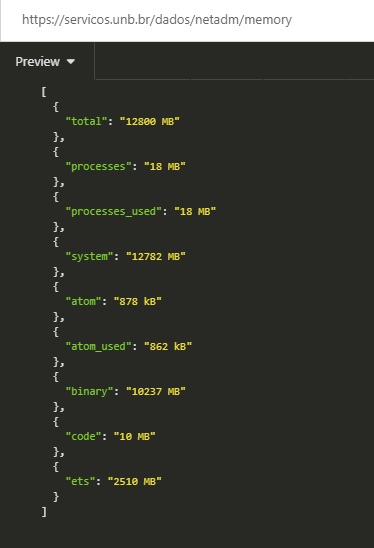
\includegraphics[scale = 0.90]{img/monitoramentoEMS.jpg}
		\caption{Serviço de consulta de utilização dos recursos de memória do Erlangms}
		\label{fun:fig:memoriaEMS}
	\end{center}
\end{figure}

\begin{figure}[h!]
	\begin{center}
	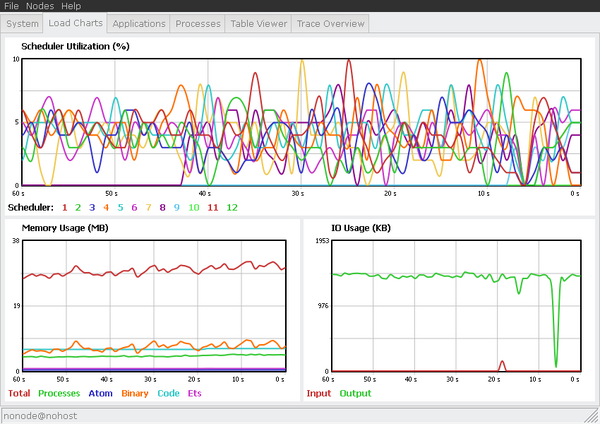
\includegraphics[scale = 0.70]{img/observerGo.jpg}
		\caption{Interface gráfica do \textit{Observer}.}
		\label{fun:fig:observer}
	\end{center}
\end{figure}

\subsection{A execução do monitoramento}

A execução do monitoramento é inciada com a integração das aplicações,ou seja quando o barramento de serviços está em funcionamento, o agente de monitoramento está ativo, assim como a ferramenta de monitoramento está ligada em modo passivo para receber as informações que são transmitidas durante a sua execução, permitindo assim a execução do monitoramento. Para representar a execução do monitoramento foi criado um \textit{design} que pode ser visualizado na figura \ref{fun:fig:arqtProjeto}. 

\begin{figure}[h!]
	\begin{center}
	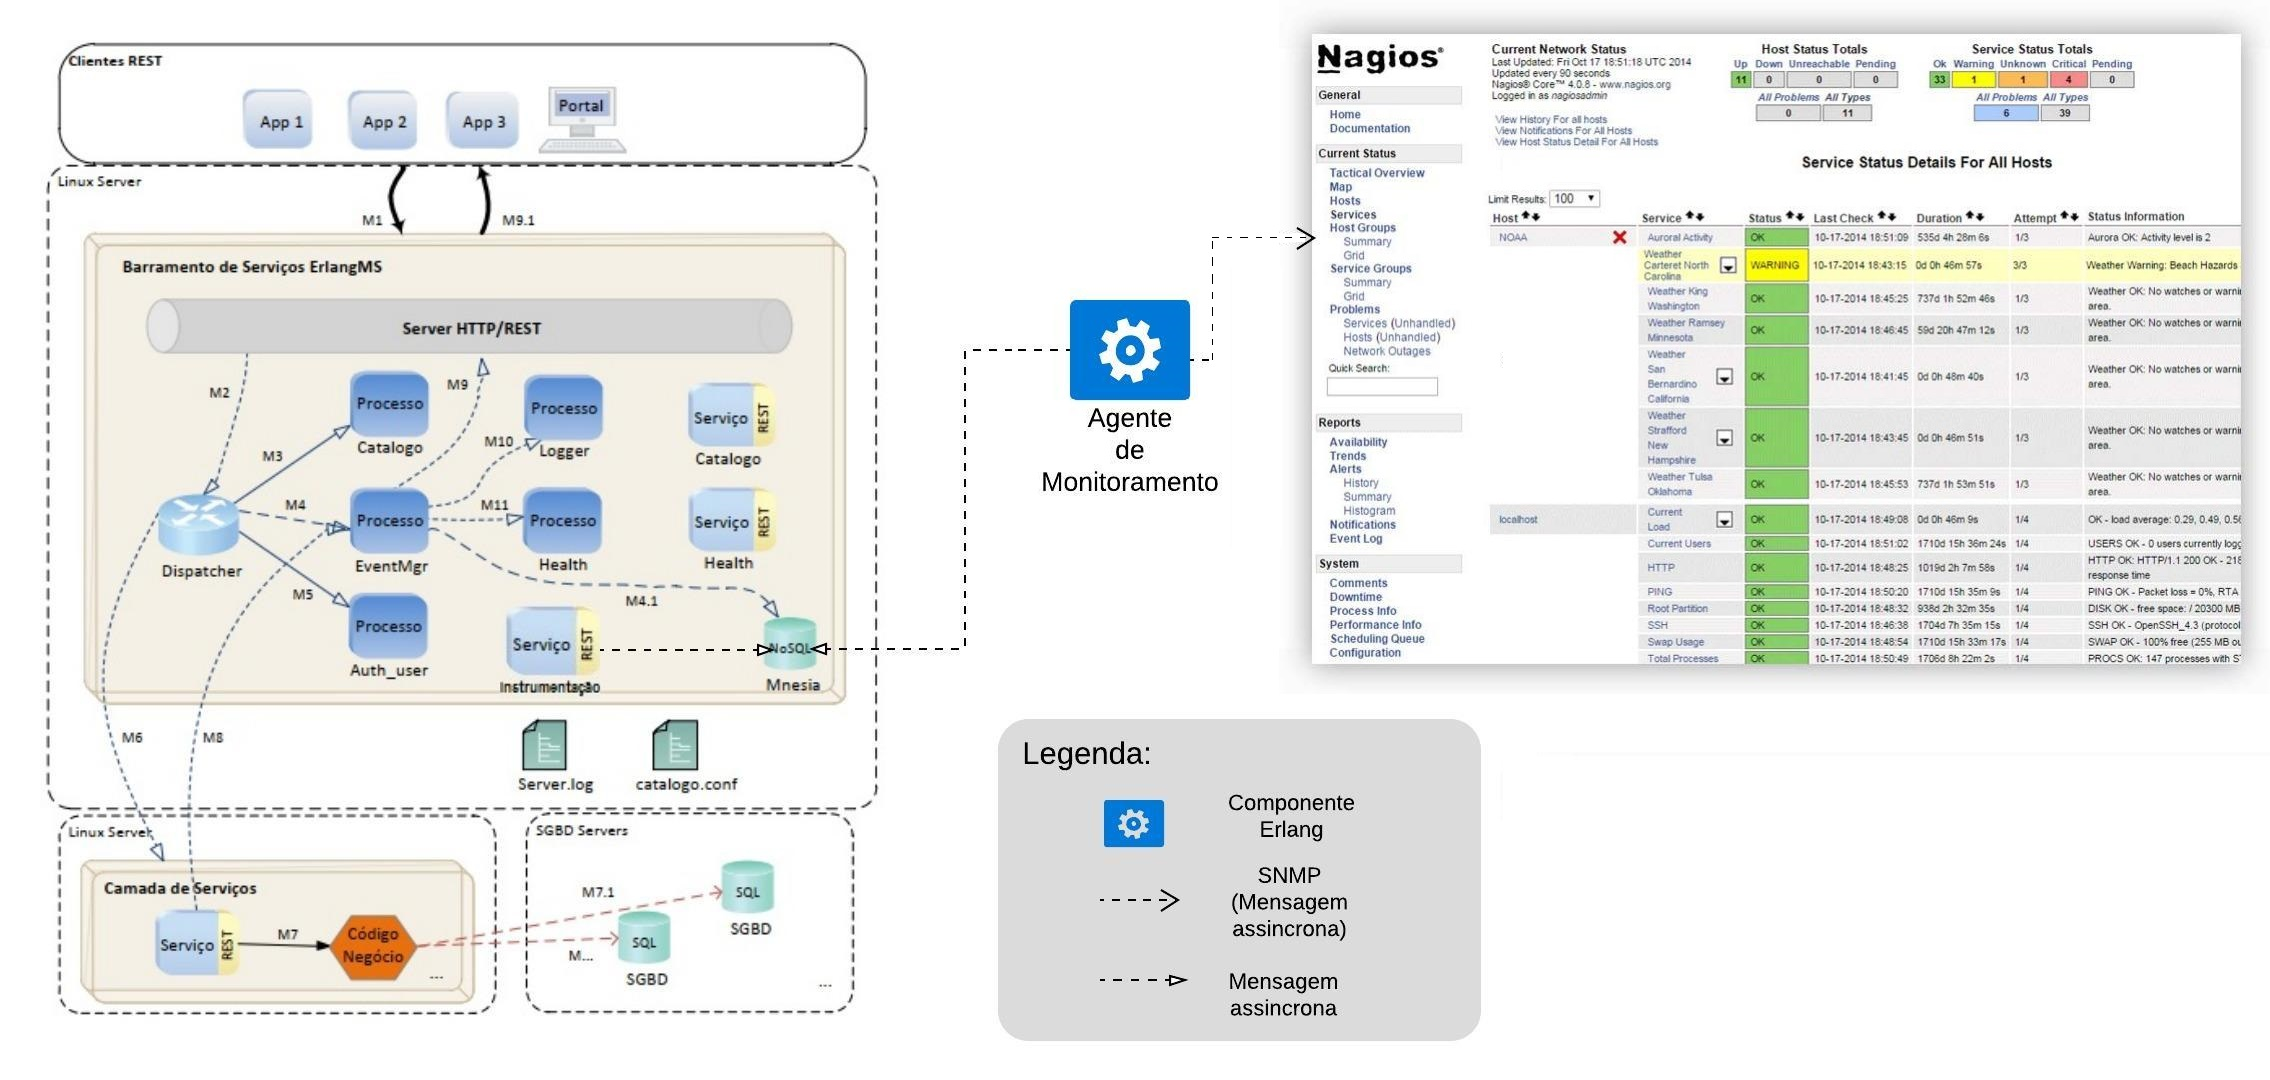
\includegraphics[scale = 0.45]{img/arqtProjeto.jpeg}
	\caption{\textit{Design} da integração das ferramentas para o monitoramento.}
	\label{fun:fig:arqtProjeto}
	\end{center}
\end{figure}



\subsection{Agente de monitoramento}

Para o acompanhamento e monitoramento serão implementados agentes de monitoramento para a realização da comunicação e notificação dos \textit{web services} monitorados. A proposta é implementar agentes para gerenciar e monitorar os \textit{web services}, a intenção é disponibilizar um serviço que seja capaz de trabalhar como uma especie de agente que informará caso haja alguma falha ou detecte um número elevado de requisições, por exemplo. A implementação dos agentes é necessária para proposta, pois é uma peça importante no monitoramento, serão os agentes de monitoramento os responsáveis para a coleta das informações que possibilitam o monitoramento dos \textit{web services}, em alguns trabalhos pesquisados os agentes foram tratados como peças fundamentais para a realização do monitoramento.       

%%%%%%%%%%%%%%%%%%%%%%%%%%%%%%%%%%%%%%%%%%%%%%%%%%%%%%%%%%%%%%%%%%%%%%%%%%%%%

\section{Protocolo SNMP}
\label{integracao_snmp}
O SNMP é o protocolo utilizado para o monitoramento de dispositivos conectados em rede. O CPD para o monitoramento dos ativos de rede utiliza, por meio de ferramentas que recebem informações desse protocolo, no entanto as ferramentas e informações fornecidas para o monitoramento servem apenas para o controle da infraestrutura de rede e servidores de aplicação, não gerenciando por exemplo, o funcionamento dos sistemas, serviços e funcionalidades das aplicações. Como proposta esse trabalho tem a intensão de fornecer e subsidiar  recursos que possibilitem o monitoramento e integração com outras ferramenta de monitoramento, para o gerenciamento de sistemas distribuídos e \textit{web services}, com a implementação de serviços que tem a responsabilidade de coletar as informações no padrão do protocolo para permitir o monitoramento dos \textit{web services}, as informações desses serviços poderão ser visualizados em qualquer ferramenta que trabalhe com os dados coletados nos padrões do protocolo.           
%\\\\\\\\\\\\\\\\\\\\\\\\\\\\\\\\\\\\\\\\\\\\\\\\


\section{Métricas de monitamento}
\label{metricas_monitoramento}

Com a implementação de serviços para gerar as informações do monitoramento, necessita-se definir um padrão ou \textit{design} para a realização da coleta, armazenamento e analise dos dados do monitoramento. Esse trabalho propõe a implementação de serviços para a realização da coleta, o desenho de um modelo de dados para o armazenamento dos dados monitorados e \textit{web services} para realização de integração com qualquer ferramenta que utilize o protocolo SNMP afim de fornecer informações para uma linguagem que permita facilmente o entendimento humano. 

%\\\\\\\\\\\\\\\\\\\\\\\\\\\\\\\\\\\\\\\\\\\\\\\\

\subsection{Desempenho}

Na literatura durante a realização da pesquisa percebeu-se a identificação de um item preocupante em relação as informações monitoradas, esse item é o desempenho, devido à quantidade de informações geradas durante o monitoramento. O trabalho tem como proposta a realização do armazenamento das informações sem problemas de desempenho, com a otimização das consultas dos serviços responsáveis pela realização e geração das informações geradas pelo monitoramento.       

%\\\\\\\\\\\\\\\\\\\\\\\\\\\\\\\\\\\\\\\\\\\\\\\\


\section{Instrumenção de código}

Este trabalho será desenvolvido por meio de seis tarefas listadas a seguir durante os períodos 2018/2 e 2019/1 que são registrados oficialmente no calendário acadêmico da UnB, e por meio do cronograma apresentado na Tabela \ref{tab:cronograma}.

	1. Escolha das abordagens que serão utilizadas por meio de características não exploradas nas soluções atuais de Implementação do protocolo SNMP para monitoramento de serviços;
  
  2. Desenvolvimento de novas abordagens que serão utilizadas na Implementação do protocolo SNMP para monitoramento de serviços ;
    
  3. Prova de conceito das abordagens desenvolvidas;
    
  4. Escrita de artigos científicos para a de submissão em congressos e periódicos;
  
  5. Escrita da dissertação de mestrado;
  
  6. Defesa do mestrado.

\begin{table}[!htpb]
	\centering
	\caption{Cronograma de execução de atividades}
	\begin{center}
		\begin{tabular}{|l|c|c|c|c|c|c|c|c|c|c|c|c|c|} \hline
Tarefa&ABR&MAI&JUN&JUL&AGO&SET&OUT&NOV&DEZ\\
			\hline
			Tarefa 1 &X&X&X& & & & & & \\
			\hline
			Tarefa 2 & & & &X&X&X& & & \\
			\hline
			Tarefa 3 & & & & &X&X&X& & \\
			\hline
			Tarefa 4 & & & & &X&X&X& & \\
			\hline
			Tarefa 5 & & & &&X&X&X&X&X \\
			\hline
			Tarefa 6 & & & & & & & & X& \\
			\hline
		\end{tabular}
		\label{tab:cronograma}
	\end{center}
\end{table} 


\fontshape{n}\selectfont%